\documentclass[border=10pt]{standalone}
\usepackage{tikz}
\usepackage{xcolor}
\usetikzlibrary{shapes.geometric, positioning}

\definecolor{entityblue}{RGB}{173, 216, 230} % light blue

\begin{document}
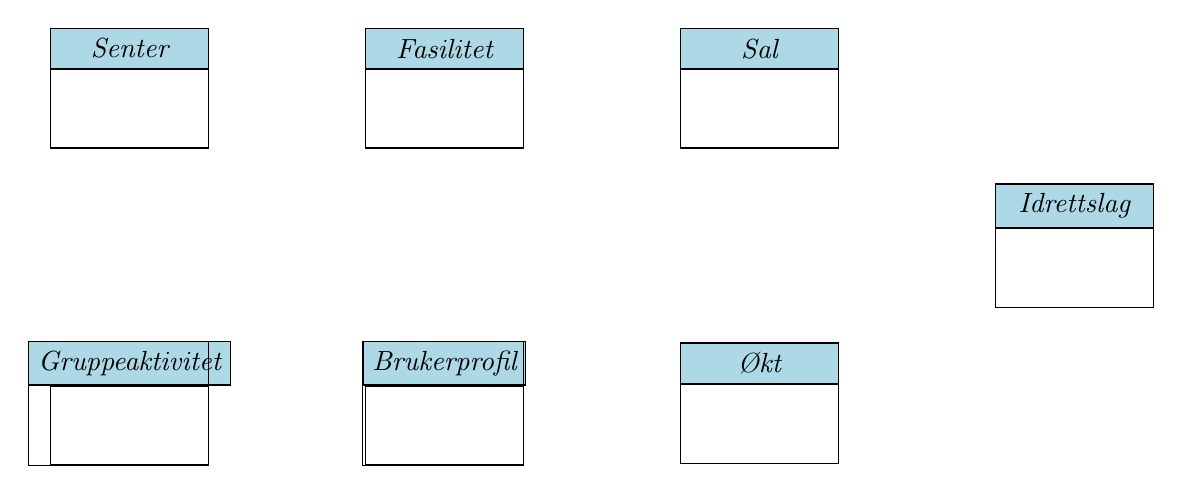
\begin{tikzpicture}[
  font=\itshape,
  entityheader/.style={
    draw=black,
    fill=entityblue,
    minimum width=2cm,
    minimum height=0.5cm,
    align=center,
  },
  entitybody/.style={
    draw=black,
    fill=white,
    minimum width=2cm,
    minimum height=1cm,
    align=left,
    inner xsep=6pt,
    inner ysep=4pt,
  },
  relationship/.style={
    draw=black,
    fill=entityblue,
    diamond,
    aspect=2,
    minimum width=1.4cm,
    minimum height=0.9cm,
    align=center,
    inner sep=2pt,
  }
]

  % Senter
  \node[entityheader] (senter-h) at (0, 4) {\normalsize Senter};
  \node[entitybody, below=0pt of senter-h] (senter-b) {};
  \draw (senter-h.south west) -- (senter-h.south east);
  \draw (senter-h.north west) rectangle (senter-b.south east);

  % Fasilitet
  \node[entityheader] (fasilitet-h) at (4, 4) {\normalsize Fasilitet};
  \node[entitybody, below=0pt of fasilitet-h] (fasilitet-b) {};
  \draw (fasilitet-h.south west) -- (fasilitet-h.south east);
  \draw (fasilitet-h.north west) rectangle (fasilitet-b.south east);

  % Sal
  \node[entityheader] (sal-h) at (8, 4) {\normalsize Sal};
  \node[entitybody, below=0pt of sal-h] (sal-b) {};
  \draw (sal-h.south west) -- (sal-h.south east);
  \draw (sal-h.north west) rectangle (sal-b.south east);

  % Gruppeaktivitet
  \node[entityheader] (gruppe-h) at (0, 0) {\normalsize Gruppeaktivitet};
  \node[entitybody, below=0pt of gruppe-h] (gruppe-b) {};
  \draw (gruppe-h.south west) -- (gruppe-h.south east);
  \draw (gruppe-h.north west) rectangle (gruppe-b.south east);

  % Brukerprofil
  \node[entityheader] (bruker-h) at (4, 0) {\normalsize Brukerprofil};
  \node[entitybody, below=0pt of bruker-h] (bruker-b) {};
  \draw (bruker-h.south west) -- (bruker-h.south east);
  \draw (bruker-h.north west) rectangle (bruker-b.south east);

  % Økt
  \node[entityheader] (okt-h) at (8, 0) {\normalsize Økt};
  \node[entitybody, below=0pt of okt-h] (okt-b) {};
  \draw (okt-h.south west) -- (okt-h.south east);
  \draw (okt-h.north west) rectangle (okt-b.south east);
  
  % Idrettslag
  \node[entityheader] (idrett-h) at (12, 2) {\normalsize Idrettslag};
  \node[entitybody, below=0pt of idrett-h] (idrett-b) {};
  \draw (idrett-h.south west) -- (idrett-h.south east);
  \draw (idrett-h.north west) rectangle (idrett-b.south east);
  
\end{tikzpicture}

\vspace{1.5cm}

\begin{tikzpicture}[
  font=\itshape,
  entityheader/.style={
    draw=black,
    fill=entityblue,
    minimum width=2cm,
    minimum height=0.5cm,
    align=center,
  },
  entitybody/.style={
    draw=black,
    fill=white,
    minimum width=2cm,
    minimum height=1cm,
    align=left,
    inner xsep=6pt,
    inner ysep=4pt,
  },
  relationship/.style={
    draw=black,
    fill=entityblue,
    diamond,
    aspect=2,
    minimum width=1.4cm,
    minimum height=0.9cm,
    align=center,
    inner sep=2pt,
  }
]
\end{tikzpicture}
\end{document}

